\section{Hardware}
Da sich das Sailwind 4.0 Projekt noch in der Entwicklung befindet, existiert noch kein komplett Zusammengebauter Prototyp in dem alle Teile des Projektes zusammenfinden. Die für diese Arbeit relevante Linearführung ist bereits als eigenstehndes Objekt zusammengebaut und wie in \autoref{fig:Systemaufbau} zusehen aufgebaut. Dabei wird die rotierende Bewegung eines BLDC Motors (Pink) mit der Hilfe eines Getriebes (Orange) und einer Gewindestange in eine Translatorische Bewegung umgewandelt, mit der der Schlitten (Hellblau) zwischen den beiden Stationären Punkten (Rot) hin und her bewegt werden kann. Die beiden Endschalter (Grün) dienen als Kollisionserkennung und können auch genutzt werden um den Bewegungsraum einzuschränken. Dabei können zwei Metallstangen (Braun) verschoben werden und geben damit vor wie viel Platz zwischen dem Schlitten und dem Stationären Elementen bleibt. Zusätzlich kann über einen Abstandssensor (dunkel Blau) die Position des Schlittens in Relation zum Abstandssensor bestimmt werden.\\

\noindent Die Linearführung soll später dazu genutzt werden um die Segel des Windkraftwerkes zu Trimmen und zu Rollen (siehe \autoref{???}). Zusätzlich zu dem präsentierten Aufbau soll sich auf dem Schlitten später ein Druckkraftsensor befinden der die Kraft auf die Rotorwelle messen soll. Dieser wurde allerdings zum Zeitpunkt der Arbeit noch nicht geliefert oder auf dem Prototypen angebracht. Getrennt vom Aufbau soll ebenfalls ein Anemometer an der Kuppel angebracht werden, das die Windrichtung und Geschwindigkeit misst.

%Hier erwähnen was Platine alles für Aufgaben hat
%Um die Segel des Windkraftwerkes jederzeit für maximale Effizienz eingestellt zu haben, müssen diese dynamisch Eingestellt werden können. Hierfür überwacht ein Controllino, die über Sensoren seine Umgebung und berechnet daraus die optimale Segel Einstellung. (KP sollte besser schon früher erwähnt werden/bzw wurde eventuell schon erwähnt)
\subsection{Ziele}
Die Hardware der Steuerung zu der eben vorgestellten Linearführung soll dabei folgende Aufgaben übernehemen:
\begin{itemize}
	\item Ansteuerung aller Sensoren und Aktoren
	\item Stromversorgung aller Komponenten
	\item Lokale Bedienung der Steuerung
	\item Ethernetkommunikation mit dem Controllino
\end{itemize}

\noindent Neben diesen Aufgaben soll die ganze Steuerung in einem zumindest Staub- und Spritzwassergeschützen Gehäuse untergebracht werden. Eine Vorgänger Gruppe hatte sich dieser Aufgabe bereits gewidmet, allerdings war der resultierende Prototyp leider nicht weiter verwendbar und hatte auch einen zu großen Formfaktor. Diese Probleme sollen in dieser Iteration ebenfalls behoben werden.

%Bei dem Entwurf der Hardware sind mehrere Dinge zu beachten. Da das Sailwind 4.0 Projekt noch in den Startschuhen steht, sind einige dieser Faktoren auch noch nicht klar Bestimmbar zum Zeitpunkt dieser Arbeit. Aus diesem Grund wurden an manchen Stellen die Design Kriterien freier oder unnötig Komplex ausgelegt.\\
%
%Um die Steuerung der Segel zu ermöglichen wird ein System benötigt das alle nötigen Akteure und Sensoren, Ansteuret und Überwacht. Hierfür soll eine Steuerelektronik Hardware entworfen werden. Da sich diese im Außeneinsatz befindet sollte diese in einem Wasserdichten Gehäuse eingeschlossen sein. Eine vorrausgehende Gruppe hatte bereits die Steuerelektronik entworfen, diese war allerdings zu groß dimensioniert und hatte einige Fehler, weswegen ebenfalls ein kleinere Formfaktor und die Behebung der Probleme als Ziel gesetzt wurden. Die Steuerelektronik soll Manuell Bedienbar sein, wewegen am Gehäuse ebenfalls eine Bedienmöglichkeit existieren sollte.

\label{Analyze_der_Aktoren_und_Sensoren}
\subsection{Analyse der bestehenden Hardware Elemente}
Um eine geeignete Steuerplatine zu entwerfen, bedarf es einer Analyse der anzusteurenden Hardware Komponenten. Diese wurden bereits von vorrausgehend Gruppen festgelegt. Diese können in die Kategorien Sensoren und Aktoren gruppiert werden. Dabei wurden die benötigte Spannung, die Stromstärke und die Schnittstellen betrachtet. Durch die Spannung und die Stromaufnahme kann später die benötigte Spurenbreite auf der Platine bestimmt werden. Die Schnittstellen geben an wie mit dem jeweiligen Gerät kommuniziert werden kann und welche davon benötigt werden.\\

\subsubsection{Sensoren}
Zu den Sensoren zählen die folgenden Komponenten:
\begin{itemize}
	\item Induktiver Endschalter: IFM IFS204
	\item Optischer Abstandssensor: IFM OGD580
	\item Anemometer: MESA WSWD
	\item Druckkraft-Sensor: Burster 8532
\end{itemize}

\noindent\textbf{Induktiver Endschalter}\newline
Zwei der IFM IFS204 Endschalter sind im Design mit eingebaut. Sie funktioneren als PNP-Schließkontakt und geben an einem Ausgang ein digitales 24V Signal aus, sobald sie ausgelöst werden. Dabei hat jeder Endschalter eine typische Stromaufnahme von <10mA und eine Betriebsspannung von 9-30V.\\

\noindent\textbf{Optischer Abstandssensor}\newline
Der Abstandssensor OGD580 funktioniert über einen Laser der vom Gerät ausgehend über eine reflektive Fläche zu diesem zurückgeworfen wird. Der Abstandsensor verfügt über ein Display das den gemessen Abstand anzeigt und über den das Gerät konfigurierbar ist. Er hat eine typische Stromaufnahme von ???mA und ebenfalls eine Betriebspannung von 9-30V. Der Abstand wird über einen digitalen Ausgang, dem sog. IO-Link ausgegeben. Da dieser typischerweise nur in der Automobilbranche zum Einsatz kommt, wurde ein zusätzlicher IO-Link Konverter hinzugefügt. Der EIO104 konvertiert die digitale IO-Link Schnittstelle zu einer Analogen 4-20mA Schnittstelle mit der einfacher Umgegangen werden kann. Dabei kommt ein zusätzlicher Stromverbrauch von ???mA hinzu.\\

\noindent\textbf{Anemometer}\\
Das WSWD Anemometer wird genutzt um die Windrichtung als auch die Windgeschwindigkeit zu messen. Dieser basiert ebenfalls auf einer 24V Versorgungsspannung und hat je nach Konfiguration und Ausführung eine Stromaufnahme von bis zu 120mA. Er besitzt ebenfalls ein Heizelement um ihn bei sehr niedrigen Temperaturen nutzen zu können. Dieses wird allerdings im Einsatzszenario und im Prototyp nicht benötigt. Die Schnittstellen des Anenometers sind abhängig von dessen Ausführung. In der zum Einsatzkommenden Ausführung, dem WSWD1, kann neben einer Analogen Schnittstelle die Daten auch über eine Digitale RS485/RS422 Schnittstelle abgefragt werden. Die Werte können Analog entweder als ein 0/4-20/24mA Strom Signal oder als ein 0/2-8/10V Spannungs Signal ausgegeben werden. Die Digitale Schnittstelle kann neben der Datenausgabe auch zur Konfiguration des Gerätes genutzt werden und bietet eine Vielzahl an Protokollen zur Kommunikation an.\\

\noindent\textbf{Druckkraft-Sensor}\newline
Der Burster Druckkraft-Sensor war der einzige Sensor der zum Zeitpunkt der Arbeit noch nicht Bestellt wurde. Dieser wurde aber dennoch mit eingeplant. Der Druckkraft Sensor kann ebenfalls mit den typischen 24V betrieben werden und hat dabei eine Stromaufnahme von ca. 12,5mA. Die Messwerte werden hier über eine Analoge 0-10V Schnittstelle übertragen.\\
\subsubsection{Aktoren}
Zu den Aktoren zählen die folgenden Komponenten:
\begin{itemize}
	\item Gleichstrommotor: Dunkermotoren BG 45x30 SI
	\item Externe Relais
\end{itemize}

\noindent\textbf{Gleichstrommotor}\newline
Der Dunkermotor BG 45x30 SI Gleichstrommotor ist das Kernelement des Aufbaus. Da der Motor eine interne Regelung besitzt hat er eine getrennte Leistungs- und Logikversorgung. Der Motor an sich wird dabei über den Leistungsteil bestromt, während über den Logikteil dieser gesteuert werden kann und Feedback bereitstellt. Die Betriebsspannung der Leistungs- und Logikversorgung sind 24V, wobei der Motor einen maximal zulässigen Dauerstrom von 3,8A ausgesetzt sein darf. Die Logikversorung hat eine Stromaufnahme von 100mA. Die Kommunikation mit dem Motor findet über vier Digitale- und einen Analogen Eingang statt. Der Motor stellt Feedback zum aktuellen Status über drei Ausgänge bereit. Diese geben die Drehrichtung, aktuelle Störungen und die Drehgeschwindigkeit des Motors an.\\
% Please add the following required packages to your document preamble:
% \usepackage{graphicx}
\begin{table}[H]
	\centering
		\begin{tabular}{|c|c|c|}
			\hline
			\textbf{Eingang 1 (IN1)} & \textbf{Eingang 0 (IN0)} & \textbf{Funktion}      \\ \hline
			0                        & 0                        & Motor aus              \\ \hline
			0                        & 1                        & Linkslauf              \\ \hline
			1                        & 0                        & Rechtslauf             \\ \hline
			1                        & 1                        & Stopp mit Haltemoment  \\ \hline
			\textbf{Eingang 3 (IN3)} & \textbf{Eingang 2 (IN2)} &                        \\ \hline
			0                        & 0                        & Drehzahlvorgabe Analog \\ \hline
			0                        & 1                        & Stromvorgabe Analog    \\ \hline
			1                        & 0                        & Geschwindigkeit 1      \\ \hline
			1                        & 1                        & Geschwindigkeit 2      \\ \hline
		\end{tabular}%
	\caption{Eingänge und Funktionen des BG 45x30 SI}
	\label{tab:digitale_Eingaenge}
\end{table}
Hier oder später noch Ein und Ausgänge definieren in Tabelle bzw. in Text erwähnen
\\

\noindent\textbf{Externe Relais}\newline
Zum Zeitpunkt der Arbeit gab es noch keinen konkreten Verwendungszweck der externen relais diese wurden für zusätzliche Funktionalitäten dennoch mit eingeplant und sollten über ein 24V Signal geschalten werden.\\

\noindent\textbf{Controllino}\newline
Der Controllino ist der zentrale Microcontroller und verwaltet alle Aktoren im System. Über diesen soll das hier zu entwerfende System, seine Befehle zur Segelausrichtung bekommen. Der Datenaustausch soll hier über eine Ethernet Schnittstelle stattfinden, um die Große Distanz zwischen Kuppel und Basis zu überbrücken.

\subsubsection{Zusammenfassung und Übersicht}
Damit sind nun alle externen anzusteurenden Komponenten abgedeckt. Die benötigte Stromversorgung sowie alle Schnittstellen sind dabei in \autoref{tab:uebersicht-externe-elemente} dargestellt. Dabei kann bereits entnommen werden, das es sehr sinnvoll ist die Platine auf ein 24V System auszulegen und diese auch mit dieser Spannung zu versorgen.
% Please add the following required packages to your document preamble:
% \usepackage{graphicx}
\begin{table}[H]
	\centering
	\resizebox{\textwidth}{!}{%
		\begin{tabular}{|l|lllllllllll|}
			\hline
			\textbf{Element} & \multicolumn{11}{l|}{\textbf{Pinout}} \\ \hline
			\textbf{Endschalter 1} & \multicolumn{1}{l|}{24V} & \multicolumn{1}{l|}{GND} & \multicolumn{1}{l|}{OUT} & \multicolumn{8}{l|}{} \\ \hline
			\textbf{Endschalter 2} & \multicolumn{1}{l|}{24V} & \multicolumn{1}{l|}{GND} & \multicolumn{1}{l|}{OUT} & \multicolumn{8}{l|}{} \\ \hline
			\textbf{Abstandssensor} & \multicolumn{1}{l|}{24V} & \multicolumn{1}{l|}{GND} & \multicolumn{1}{l|}{IO-Link} & \multicolumn{8}{l|}{} \\ \hline
			\textbf{IO-Link Konveter} & \multicolumn{1}{l|}{24V} & \multicolumn{1}{l|}{GND} & \multicolumn{1}{l|}{AOUT} & \multicolumn{8}{l|}{} \\ \hline
			\textbf{Anemometer} & \multicolumn{1}{l|}{24V} & \multicolumn{1}{l|}{GND} & \multicolumn{1}{l|}{AOUT} & \multicolumn{1}{l|}{AOUT} & \multicolumn{1}{l|}{AGND} & \multicolumn{1}{l|}{RS485+} & \multicolumn{1}{l|}{RS485-} & \multicolumn{4}{l|}{} \\ \hline
			\textbf{Druckkraftsensor} & \multicolumn{1}{l|}{24V} & \multicolumn{1}{l|}{GND} & \multicolumn{1}{l|}{AOUT} & \multicolumn{1}{l|}{AGND} & \multicolumn{7}{l|}{} \\ \hline
			\textbf{Motor Leistung} & \multicolumn{1}{l|}{24V} & \multicolumn{1}{l|}{GND} & \multicolumn{9}{l|}{} \\ \hline
			\textbf{Motor Logik} & \multicolumn{1}{l|}{24V} & \multicolumn{1}{l|}{GND} & \multicolumn{1}{l|}{IN0} & \multicolumn{1}{l|}{IN1} & \multicolumn{1}{l|}{IN2} & \multicolumn{1}{l|}{IN3} & \multicolumn{1}{l|}{AIN} & \multicolumn{1}{l|}{AGND} & \multicolumn{1}{l|}{OUT1} & \multicolumn{1}{l|}{OUT2} & OUT3 \\ \hline
			\textbf{Externes Relais 1} & \multicolumn{1}{l|}{OUT} & \multicolumn{1}{l|}{GND} & \multicolumn{9}{l|}{} \\ \hline
			\textbf{Externes Relais 2} & \multicolumn{1}{l|}{OUT} & \multicolumn{1}{l|}{GND} & \multicolumn{9}{l|}{} \\
			\hline
			\textbf{Controllino} & \multicolumn{1}{l|}{Ethernet} & \multicolumn{10}{l|}{} \\ \hline
		\end{tabular}%
	}
	\caption{Übersicht Stromversorgung und Schnittstellen der externen Elemente}
	\label{tab:uebersicht-externe-elemente}
\end{table}
\subsection{Auswahl der Platinen Bauteile}
Da nun klar ist welche Anforderungen durch die anzuschließenden Geräte bestehen, kann auf Basis dieser nun weiterverfahren werden. Dabei soll im folgenden ein geeigneter Mikrocontroller, sowie die nötigen Platinenkomponenten ausgewählt werden, um mit den Hardwarekomponenten zu kommunizieren und diese mit Strom zu versorgen.
\subsubsection{Mikrocontroller}
Die Auswahl des Mikrocontrollers wurde auf der Basis folgender Kriterien beschlossen:
\begin{itemize}
	\item Benötigte Inputs und Outputs
	\item Softwaresupport 
	\item Entwicklung
	\item Verfügbarkeit
\end{itemize}
Dabei gab es die Option den Chip als einzelnes Element direkt auf die selbst erstellte Platine einzubetten oder ein Entwicklungsboard als Basis zu nutzen und eine Erweiterungsplatine dafür zu nutzen. Es wurde sich dabei für ein Entwicklungsboard entschieden um bereits parallel zum Hardwaredesign eine geeignete Software zu entwickeln und diese bereits mit einem Prototypischen Aufbau zu testen (Vielleicht noch erwähnen, probleme bei vorheriger Gruppe). Dies bietet ebenfalls den Vorteil, das beim zerstören des Chips ein schneller Ersatz angebracht werden kann und auch bereits ein Formfaktor vorgegeben ist. Auch kann durch den bereits angebrachten Debugger, schneller neue Software getestet und aufgespielt werden. Ebenfalls besitzen viele Entwicklungsboards bereits einen Ethernetport der sowieso benötigt wird.\\

\noindent Durch die oben genannten Kriterien und die Entscheidung ein Entwicklerboard zu benutzen viel die Wahl auf das STM32 NUCLEO F439zi Board. Diese waren bereits an der HTWG Konstanz Verfügbar, sind durch den Softwaresupport von ST und ihrer eigenen Entwicklungsumgebung einfach zu Programmieren und Aufzusetzen. Außerdem bieten ihre Entwicklungsboards einen abbrechbaren Debugger und das Board kann damit auch außerhalb der Entwicklungsphase eingesetzt werden.
\subsubsection{Relais}
Um das auslösen eines Endschalters an den Mikrocontroller weiterzugeben, werden zwei 24V Relais genutzt die bei der Aktivierung der Spule ein 3,3V Signal an den Eingang des Mikrocontrollers weitergeben. Gleichzeitig wird durch das Umschalten des Relais der Eingang 1 oder 2 des Motors auf Null gesetzt. Diese geben die Drehrichtung an und stoppen den Motor sobald beide auf Null gesetzt sind. Da dieses System unabhängig von der Software des Mikrocontrollers agiert, dienen diese gleichzeitig als Ausfallsichere Aktoren.
\subsubsection{Optokoppler}
Um die restlichen 24V Aus- und Eingänge zu steueren oder auszulesen kommen Optokoppler zum Einsatz. Diese isolieren ähnlich zu Relais den 24V und 3,3V Schaltkreis und ermöglichen es durch einen kleinere Spannung eine größere Last zu schalten. Dabei werden insgesamt 9 benötigt um die digitalen Ein und Ausgänge des Motors und die beiden externen Relais zu schalten. Da es sich beim Ausgang 3? des Motors um ein Pulsierendes Signal zur Ermittelung der Drehgeschw. des Motors handelt wurde auf eine schnelle Schaltzeit der Optokoppler geachtet (hier Berechnung einfügen).
\subsubsection{RS485 zu UART Konverter}
Um das Anemometer über die RS485 Schnittstelle zu konfigurieren und Daten abzufragen wird ein zusätzlicher Baustein benötigt. Dieser Konvertiert das differenzielle RS485 Signal zu einem nicht differenziellen \ac{UART} Signal, das der Mikrocontroller untertsützt.
\subsubsection{FRAM}
Da die neutrale Position des Segels dauerhaft gespeichert werden soll, wird ein nicht flüchtiger Speicherstein benötigt. Dabei ist der \ac{FRAM} einer der billigsten Speichermöglichkeiten für diesen Zweck. Es wurde die geringste Speichergröße gewählt, da die gespeicherten Daten jederzeit überschrieben werden kann. Der FRAM wird über \ac{SPI} angesteuert.
\subsubsection{Operations Verstärker}
Um die Drehzahl des Motors vorgeben zu können, wird ein Analoges Signal im Bereich von 0-10V benötigt. Da der Mikrocontroller bei einer Versorgungsspannung von 5V maximal ein Analoges Signal von 3,3V Ausgeben kann, wird ein Operationsverstärker benötigt. Dieser soll mit der 24V Versorgungsspannung das Ausgangssignal auf bis zu 10V skalieren.
\subsubsection{DC/DC-Wandler}
Um alle Komponenten zu versorgen Bedarf es insgesamt 3 verschieden Spannungspotenzialen: 24V, 5V und 3,3V. Um dies zu erreichen sollen alle externen Komponenten direkt mit den 24V versorgt werden. Der Mikrocontroller soll mit den 5V versorgt werden, da er somit auch ohne Debugger Erweiterung genutzt werden kann. Hierfür wird ein Step Down konverter genutzt der die 24V Versorgungsspannung auf 5V herunterbricht. Die 5V sollen daraufhin auf weitere 3,3V heruntergebrochen werden, um die sonstigen Bauteile mit dieser zu Versorgen.
\subsubsection{Strom Sensor}
Zur Überwachung des Motor Stroms kommt ein Hallstromsensor zum Einsatz. Dieser wird kontiniuerlich abgefragt und kann bei einem zu großem Stromfluss z.B größer als 3,8A den Motor stoppen oder Warnungen Ausgeben.
\subsubsection{Konnektoren}
Die externen Komponenten sollen über Schraubklemmen direkt an die Platine angeschlossen werden. Je nach Querschnitt der Kabel wurde ein größeres oder kleineres Rastermaß gewählt um Platz auf der Platine einzusparen.
\subsubsection{Analoge Eingänge}
Um die Analogen Ausgänge des Abstandsensors und des Anemometers auszulesen wird das 4-20mA Stromsignal über einen Widerstand zu einem 0-3V Spannungssignal gewandelt das mit dem \ac{ADC} des Microcontrollers gelesen werden kann.
\subsection{Gehäuse und Befestigung}
Um die Platine die sich später in der Kuppel befinden soll, vor z.B Staub und Wasser zu schützen soll diese in einem Gehäuse untegebracht werden. Das Gehäuse sollte vorallem im Innenraum genug Platz bieten um Kabel an der Platine zu befestigen, eine Möglichkeit bieten die Platine darin zu befestigen und genug Platz auf der Oberfläche bieten um die Bedienoberfläche und die unterschiedlichen Kabel Durchführungen zu positionieren.
\subsection{Platinen Schaltplan}
\begin{figure}[H]
	\centering
	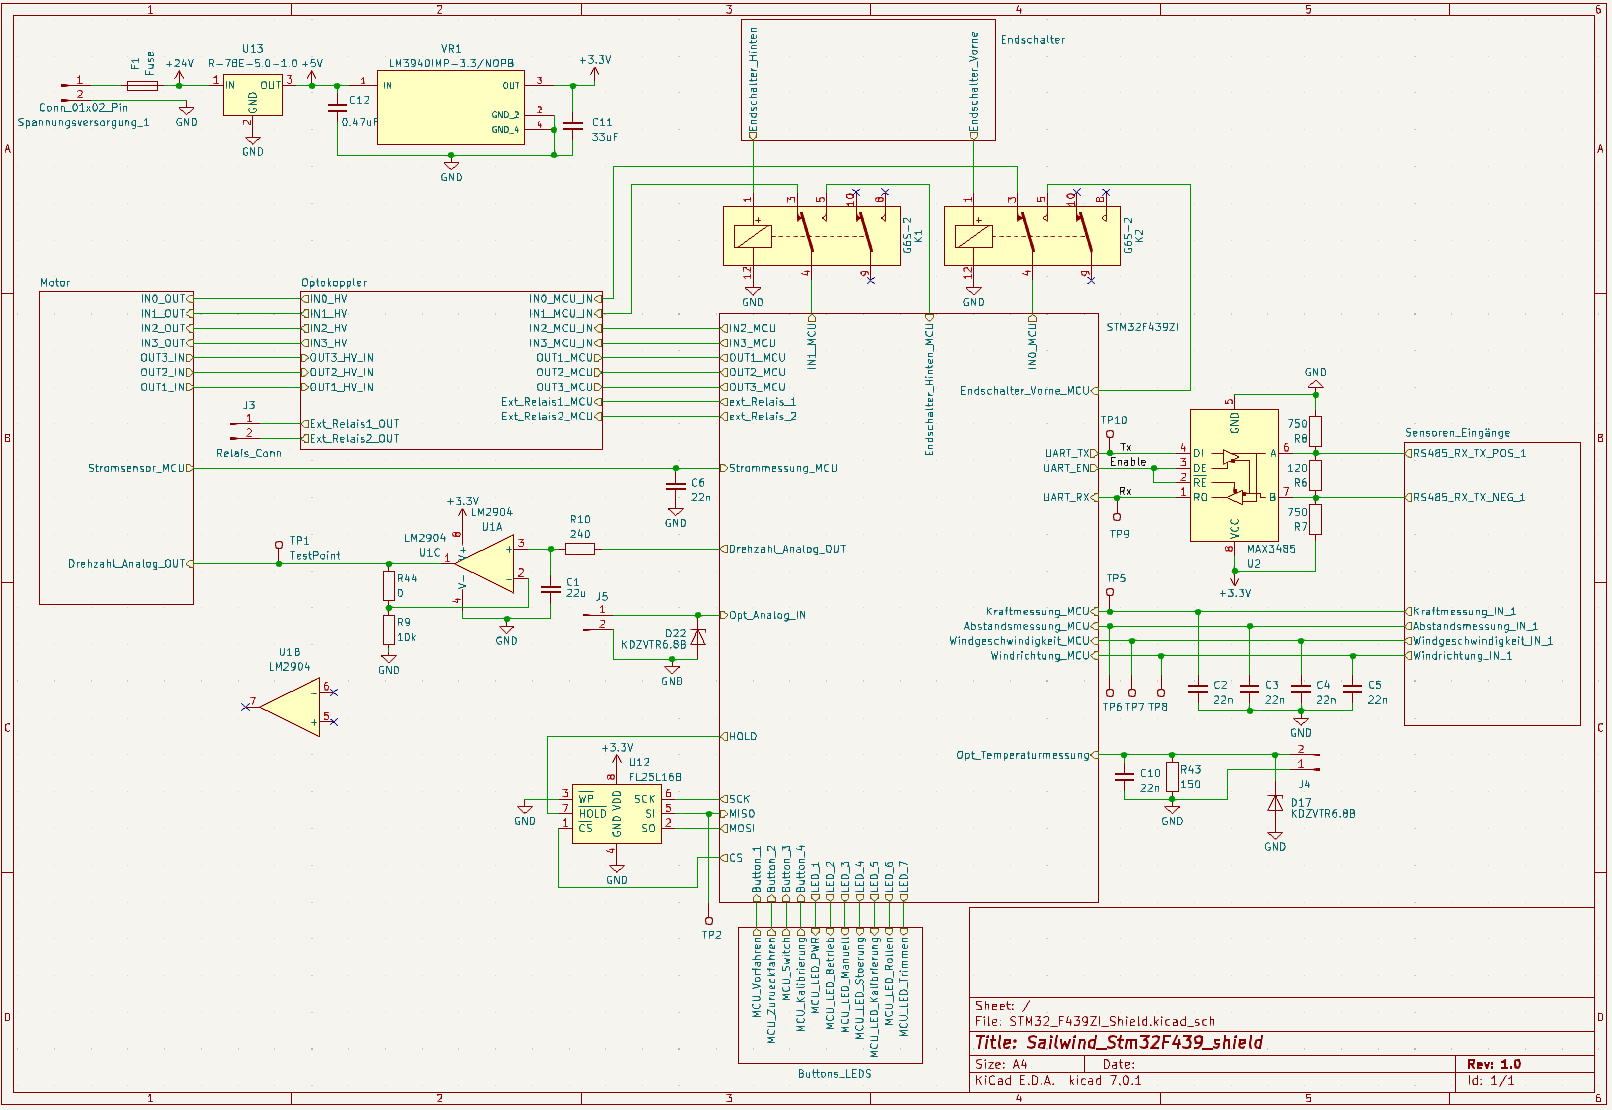
\includegraphics[width=1.0\textwidth]{images/Hardware/Schaltplan_Gesamt.PNG}
	\caption{Gesamtschaltplan der Platine}
	\label{fig:Schaltplan_gesamt}
\end{figure}
Der komplette Schaltplan ist in \autoref{fig:Schaltplan_gesamt} dargestellt und ist ebenfalls im Anhang \autoref{Anhang_Schaltplan} zu finden. Der Schaltplan ist in unterschiedliche Bereiche eingeteilt die die Gruppierung der Komponenten wiedergibt. Dabei ist das STM32F439zi Entwicklerboard zentral Positioniert und alle Bauteile und Komponeten um dieses verteilt. Bauteile die nur einfach Verbaut sind wie z.B der FL25L16B \acs{FRAM} (Unten Links) wurden nicht in Gruppen eingeteilt sondern direkt in der Gesamt Ansicht Positioniert. Dasselbe gilt auch für die Puffer Kondensatoren an den Analogen Aus- und Eingängen. Oben Links befindet sich die Spannungsversorgung der Platine und die \acs{DC}/DC Wandler. Überhalb des STM32 befinden sich die beiden Relais die an die Endschalter verbunden sind. Links außen befindet sich der \ac{BLDC} Motor der mit dem Operationsverstärker und den Optokoppler verbunden ist. Rechts befinden sich alle Analogen Sensoren, bis auf den Stromsensor. Dort ist ebenfalls der MAX3485 \acs{UART} Konvertierer zu sehen. Unterhalb des Mikrocontrollers befinden sich die Knöpfe und LEDS die das \acs{HMI} bilden. Im folgenden sollen exemplarisch die Motor, Oktokoppler und 
\subsubsection{STM32F439zi Gruppe}
Die STM32F
\subsubsection{Motor Gruppe}
\begin{figure}[H]
	\centering
	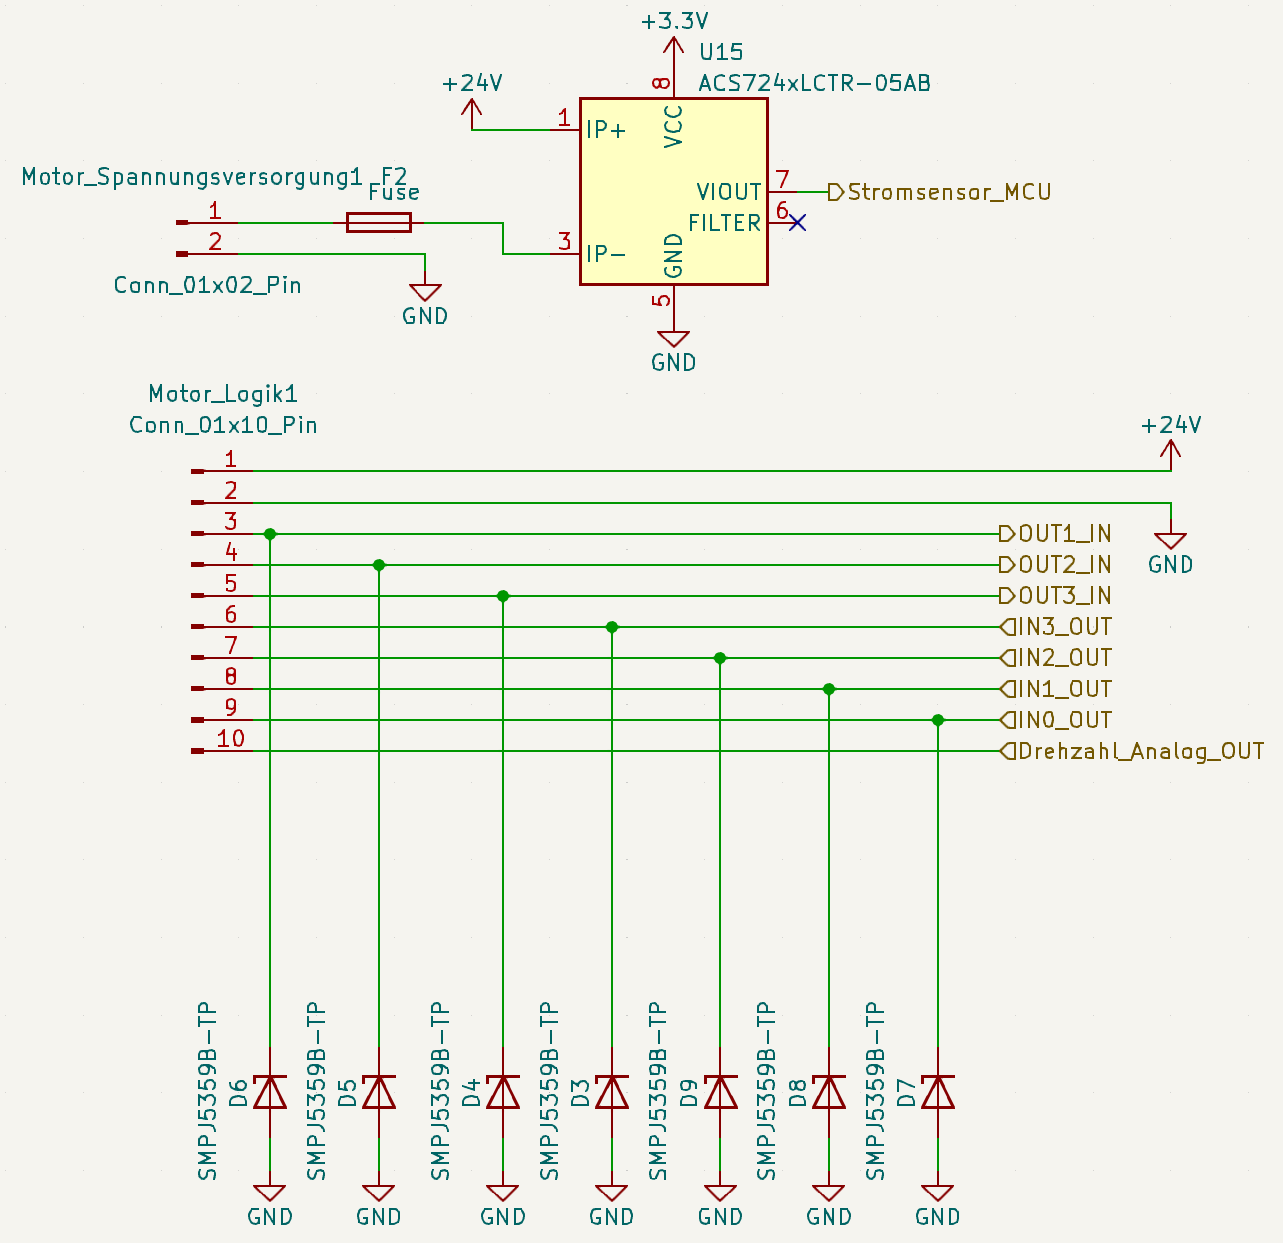
\includegraphics[width=1.0\textwidth]{images/Hardware/Motor_Schaltplan.PNG}
	\caption{Schaltplan der Motorgruppe}
	\label{fig:Motor_gruppe}
\end{figure}

\subsubsection{Optokoppler Gruppe}
\begin{figure}[H]
	\centering
	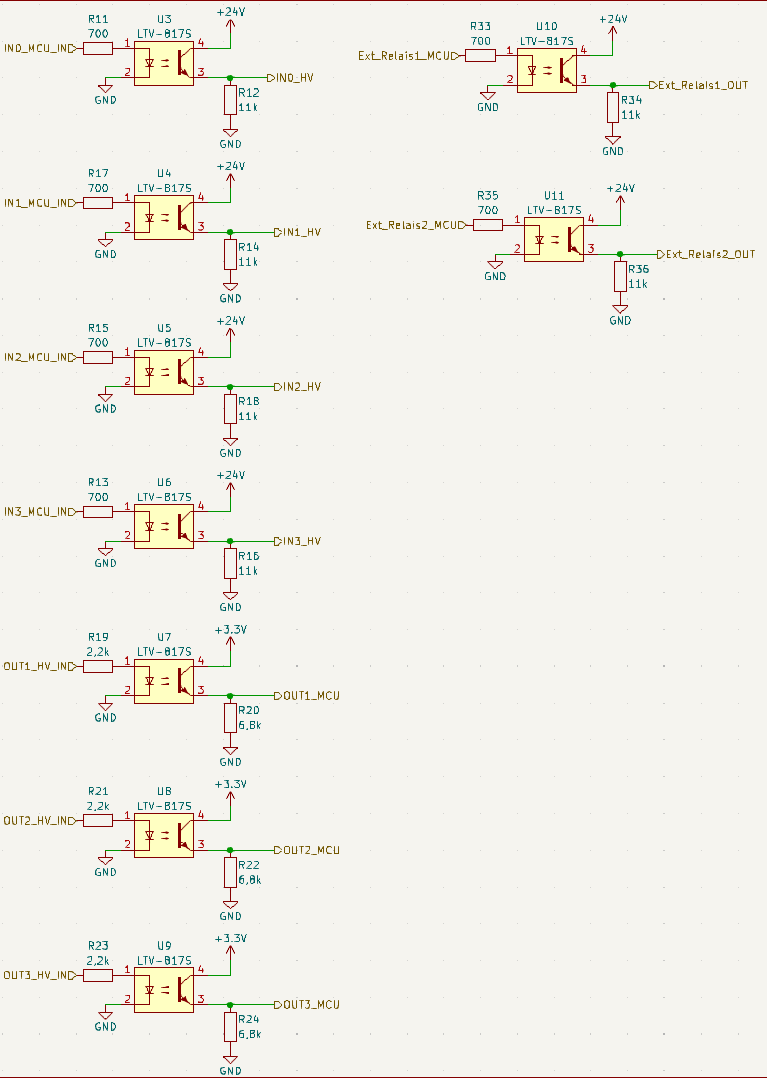
\includegraphics[width=1.0\textwidth]{images/Hardware/Optokoppler_Schaltplan.PNG}
	\caption{Schaltplan der Optokopplergruppe}
	\label{fig:Optokoppler_gruppe}
\end{figure}
Die Optokoppler sind alle gleich Aufgebaut. Der Eingangswiderstand (links) begrenzt den Strom der im inneren verbauten LED auf eine laut Datenblatt spezifizierten Strom begrenzt. Ein Pulldown Widerstand auf der Ausgangsseite begrenzt den maximal erlaubten Strom zum Mikrocontroller.
\subsubsection{Endschalter Gruppe}
\begin{figure}[H]
	\centering
	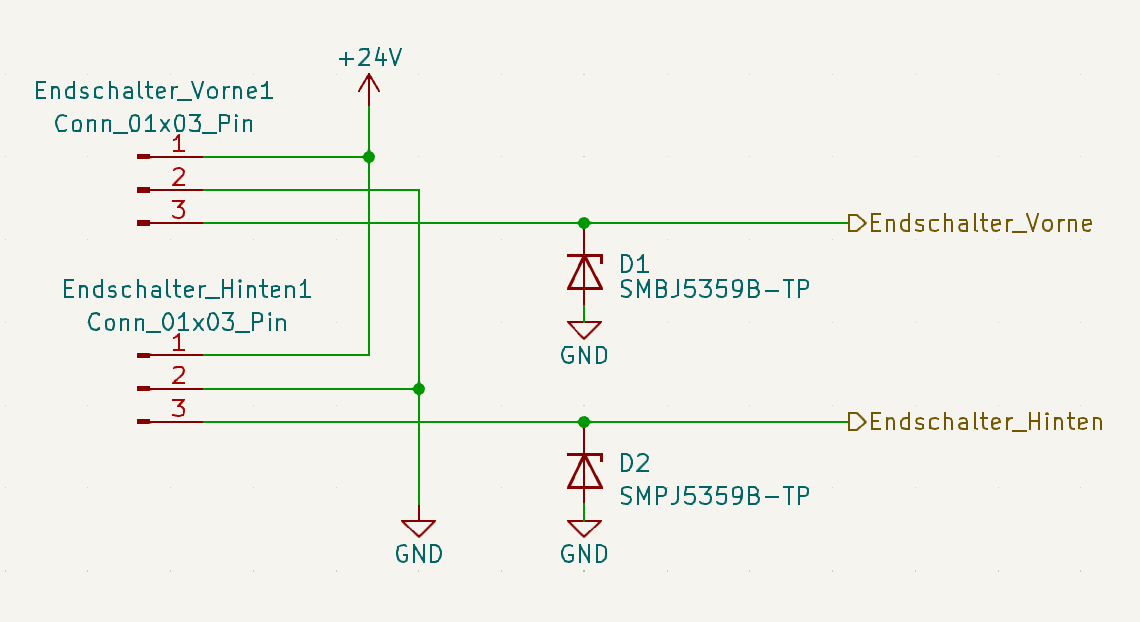
\includegraphics[width=1.0\textwidth]{images/Hardware/Endschalter_Schaltplan.PNG}
	\caption{Schaltplan der Endschaltergruppe}
	\label{fig:Endschalter_gruppe}
\end{figure}
\subsubsection{Sensoren Gruppe}
\begin{figure}[H]
	\centering
	\includegraphics[width=1.0\textwidth]{images/Hardware/Sensoren_Eingänge_Schaltplan.PNG}
		\caption{Schaltplan der Buttons und LEDs}
	\label{fig:Sensoren_Gruppe}
\end{figure}
\subsubsection{Buttons und LEDs Gruppe}
\begin{figure}[H]
	\centering
	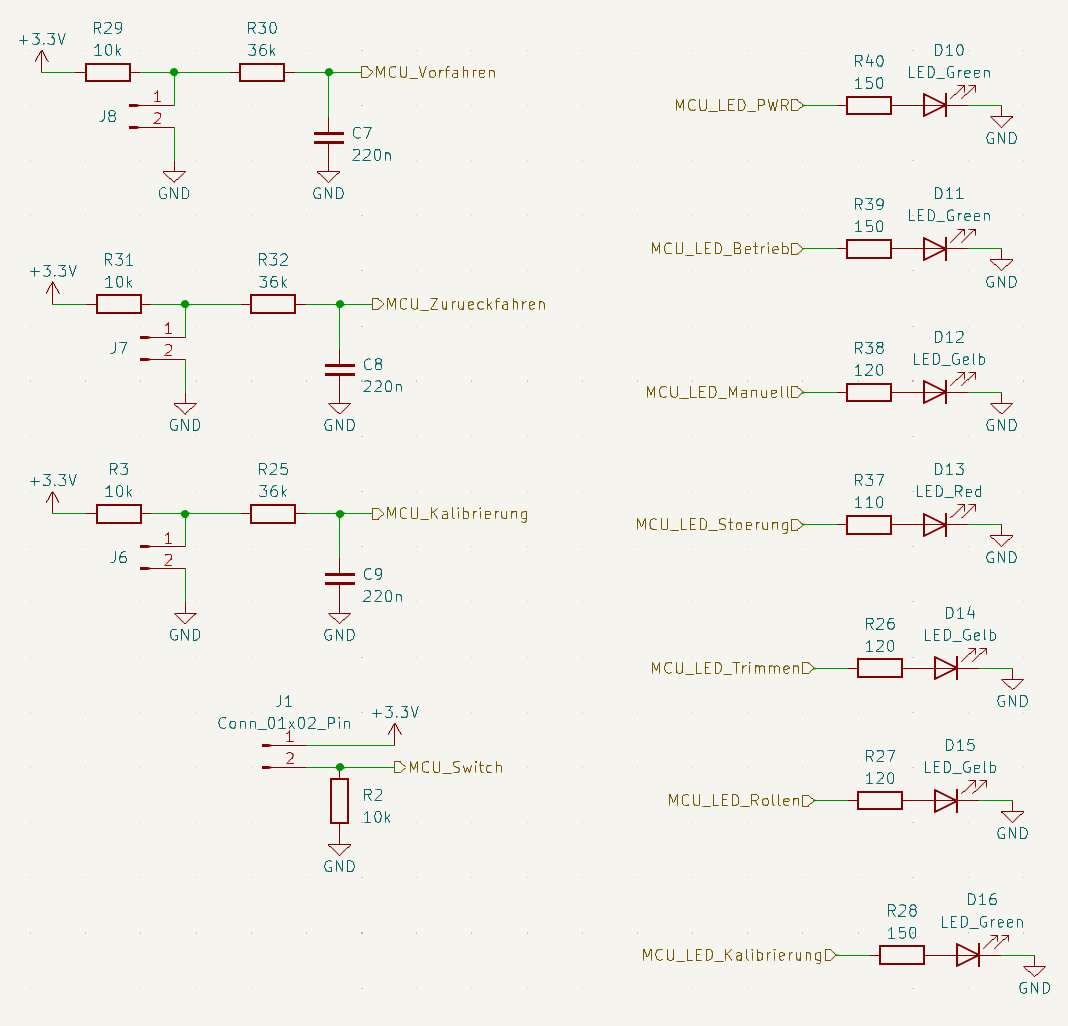
\includegraphics[width=1.0\textwidth]{images/Hardware/LEDS_und_buttons_schaltplan.PNG}
	\caption{Schaltplan der Buttons und LEDs}
	\label{fig:HMI_Gruppe}
\end{figure}
\subsection{\ac{PCB}}
\begin{figure}[H]
	\centering
	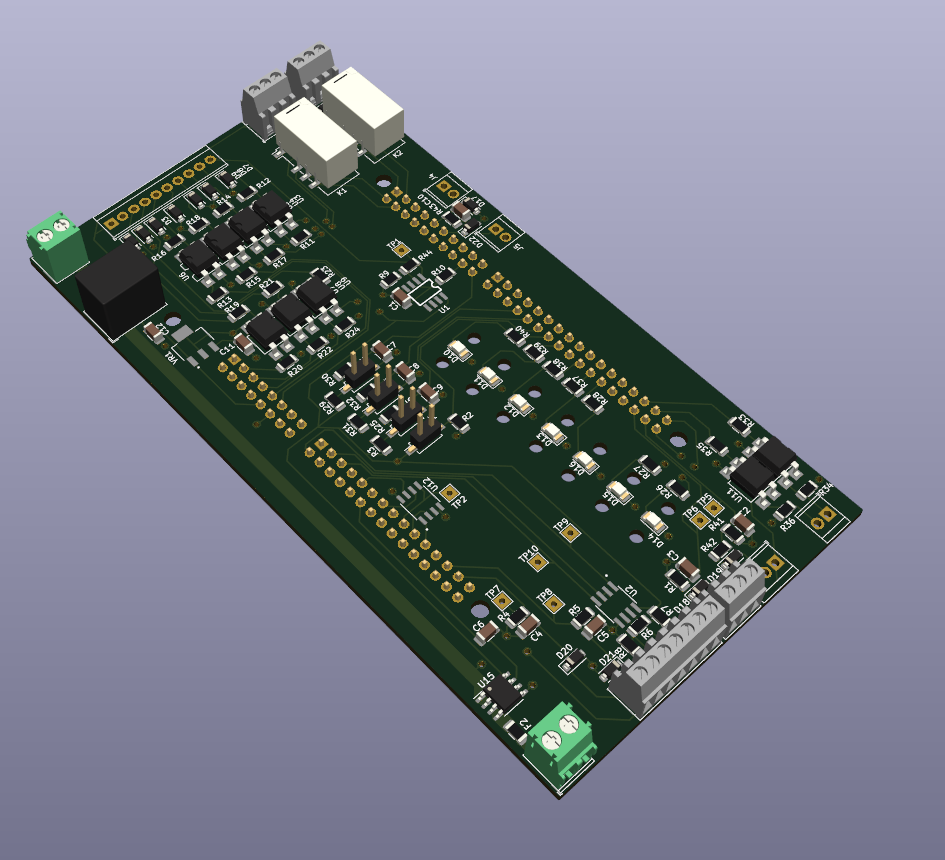
\includegraphics[width=1.0\textwidth]{images/Hardware/Platine_Fertig_3D_ansicht(1).PNG}
	\caption{3D Ansicht des fertigen PCBs}
	\label{fig:PCB_3D}
\end{figure}
\subsection{\ac{HMI}}
Das HMI besteht aus einer Reihe von Kippschaltern, Knöpfen und LEDs. Diese sind sind in \autoref{fig:Bedienung} dargestellt. Dabei soll die gewünschte Neutrale Position der Linearführung durch einen Manuellen Betrieb stattfinden. Dabei kann der Endnutzer über die Trimm und Roll Knöpfe zum gewünschten Mittelpunkt Navigieren und diesen mit dem dritten Knopf speichern. Anschließend kann mittels des Kippschalters in den Automatik Betrieb gewechselt werden in dem das betätigen der Knöpfe ignoriert wird.
Eine Reihe von LEDs gibt Feedback über den aktuellen Zustand der Linearführung. Dabei wird konstant der aktuelle Betriebsmodus durch zwei LEDs angegeben. Ebenfalls wird die Position relativ zur festgelegten neutral Position durch zwei gelbe LEDs angegeben. Eine Störung in der Steuerung oder im Motor wird durch eine rote LED angegeben.\\
Die Knöpfe und Kippschalter sind beide am Gehäuse montiert und sind Spritzwasser geschützt. Im Gegensatz dazu sind die LEDs direkt auf der Platine platziert und werden durch flexible Lichtleiter zur Außenseite des Gehäuses geführt.
\begin{figure}[H]
	\centering
	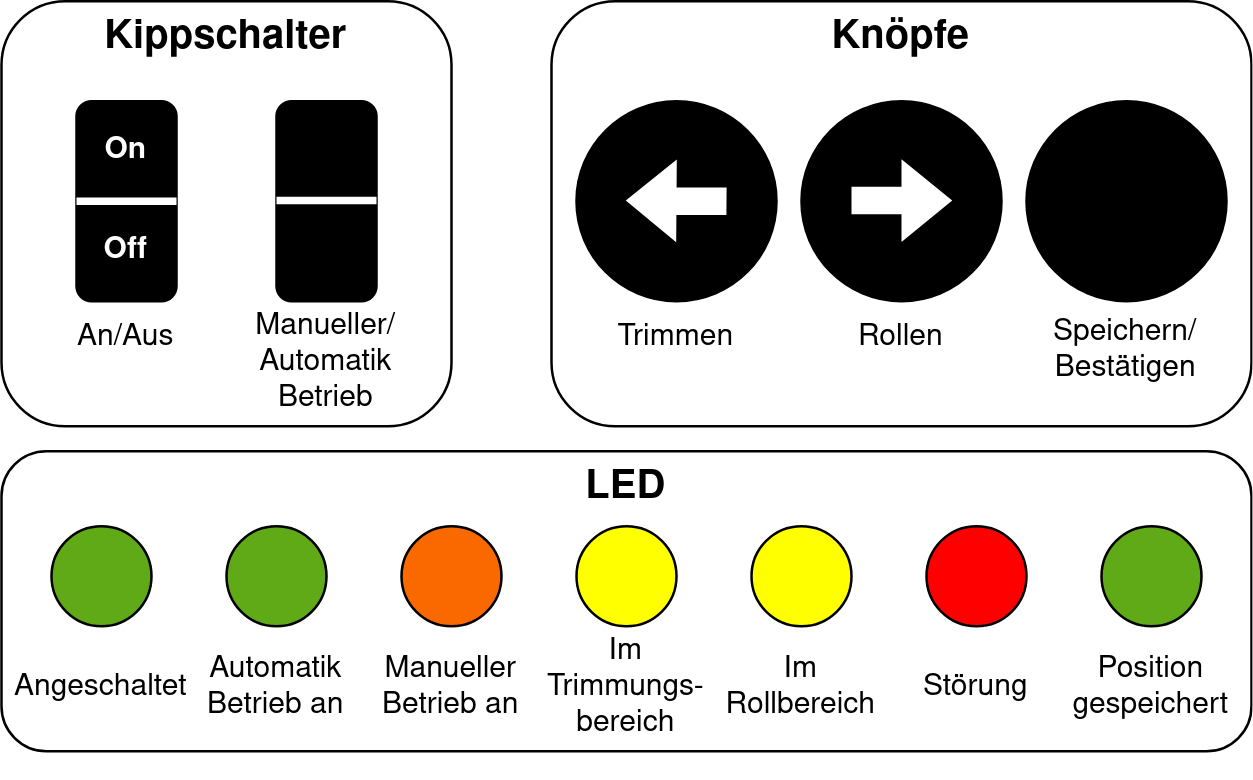
\includegraphics[width=1.0\textwidth]{images/Hardware/Bedienung.drawio.png}
	\caption{HMI der Segel Steuerung}
	\label{fig:Bedienung}
\end{figure}

\subsection{Probleme}
Während der Nutzung und Bestückung des \ac{PCB}s sind einige Probleme aufgetreten. Diese waren auf das Design oder falsche Berechnungen zurückzuführen. Diese sollen im folgenden erklärt und korrigiert werden.
\subsubsection{Schraubklemmen Löcher}
Der erste Fehler der zu Beginn auffiel, war der Durchmesser der Löcher für die Schraubklemmen. Diese waren zwar groß genug dimensioniert um die Pins Schraubklemmen durchzuführen, aber waren nicht darauf angepasst Nieten einzufügen um die Pins elektrisch mit der Platine zu verbinden. Die Löcher waren ebenfalls zu klein um mit Drähten eine elektrische Verbindung zwischen dem Pin und dem Board herzustellen. Dies führte zu vielen elektrischen Kontakt Problemen und minderte die horizontale Stabilität der Schraubklemmen. Die Kontakt Probleme führten auch zur mangelnden Präzision der Analog Eingänge (siehe \autoref{Mangelnde_Präzision}).
\subsubsection{Operationsverstärker}
Der Operationsverstärker war zwar als Verstärkerschaltung richtig konfiguriert, allerdings musste die Verstärkerspannung von 3,3V auf 24V angehoben werden, um die 10V zu erreichen. Zusätzlich wurde der Spannungsteiler am Ausgang des OPVs entfernt und der erste Widerstand gegen einen 0Ohm Widerstand getauscht.
\subsubsection{RS485 Bias Widerstände}
Die RS485 Widerstände wurden anfänglich die empfohlenen Widerstände in der WSWD Dokumentation genutzt. Hier wurde bei einer Versorgungsspannung von 5V ein Busabschlusswiderstand $R_t$ von 120$\Omega$ und zwei Biaswiderstände $R_b$ von 750$\Omega$ empfohlen (vgl.\cite{WSWD} S.21). Dies sorgte allerdings für eine zu große Differenz der beiden Spannungen und der MAX3485 konnte nicht zwischen high und low unterscheiden. Deshalb wurde stattdessen nach der Anleitung des MAX3485 die Differenz zwischen beiden Potenzialen auf 0,2V begrenzt. Hierfür wurde auf die Berechnung in dem von Texas Instruments veröffentlichten Bericht: \glqq{}RS-485 failsafe for an idle bus\grqq{} zurückgegriffen. Hier lässt sich anhand der Formel: 
\begin{equation}
	R_b = (\frac{V_s}{V_{diff }}+1)\times27,8\Omega
\end{equation}
die beiden Bias Widerstände für das RS-485 Netzwerk berechnen. Dabei kam für die Eingesetzten Werte:
\begin{equation}
	R_b = (\frac{3,3V}{0,2V}+1)\times27,8\Omega = 486,5\Omega
\end{equation}
Der nächst kleinere Widerstand der Verfügbaren E24 Reihe wurde dann auf 470$\Omega$ gewählt. Damit konnte daraufhin erfolgreich über RS485 kommuniziert werden.
\subsubsection{FRAM Anschlüsse}
Die SPI Anschlüsse des FRAM Speicher wurden falsch verbunden dabei wurden die MOSI und MISO Leitung vertauscht was 
\subsubsection{Präzision der Analogen Signale}
Klemmenlöcher
Operationsverstärker
Widerstände RS485
FRAM MOSI/MISO
Präzison Analog Eingänge